\chapter{Approccio terapeutico al linfoma non Hodgkin}

L’approccio terapeutico al linfoma non-Hodgkin, dipende da diversi fattori: dal sottotipo di linfoma, 
dallo stadio della malattia, dal possibile coinvolgimento extranodale, dall’eventuale presenza di sintomi come febbre, 
sudorazione notturna, perdita di peso superiore al 10\% negli ultimi sei mesi\cite{LLS}.

\section{"Watch and wait"}
L’approccio “watch and wait” viene scelto per pazienti con linfoma indolente, che non presentano sintomi e che 
alla diagnosi mostrano un’estensione della patologia limitata. 
Si tratta di un’osservazione attenta nel corso del tempo, mediante analisi ed esami mirati\cite{LLS}.\\
Alcuni studi, hanno mostrato, come non ci fosse una differenza a livello di sopravvivenza, tra i pazienti che venivano 
fin da subito sottoposti a trattamento, rispetto a chi invece veniva osservato nel tempo; l’approccio da scegliere 
viene concordato tra il medico e il paziente, in quanto ogni caso è a sé e deve essere valutato singolarmente\cite{LLS}.\\
Per alcuni pazienti la malattia può restare stabile o progredire lentamente per molti anni, 
per altri può evolvere in forme aggressive di linfoma, che necessita di trattamento tempestivo.\\
Per pazienti con linfoma aggressivo, si ha un approccio di polichemioterapia basata su schemi terapeutici 
che associano farmaci chemioterapici, corticosteroidi e anticorpi monoclonali.\\ 
Per quel che riguarda la chemioterapia, sarà approfondita in un capitolo a parte.\\ 
In questo capitolo ci concentreremo su altri approcci terapeutici: 
radioterapia, immunoterapia, trapianto autologo e allogenico di cellule staminali emopoietiche.

\section{Radioterapia}
La radioterapia usa radiazioni ad alte dosi, per distruggere le cellule cancerose o per rallentare la loro crescita. 
Essa può essere esterna o interna e quest'ultima è detta anche brachiterapia. 
La caratteristica della radioterapia esterna è che è un trattamento localizzato, cioè rivolto alla sola parte 
del corpo interessata dal tumore. 
Per quanto riguarda la radioterapia interna, possiamo parlare di brachiterapia o di radioterapia sistemica. 
La brachiterapia è un trattamento locale, quindi di una specifica parte del corpo, in cui particelle contenenti 
radiazioni vengono immesse nel tumore o nelle sue vicinanze. 
La radioterapia sistemica è così definita perché il trattamento è immesso nel corpo per via orale, endovenosa o 
tramite iniezione e in questo modo vengono raggiunti tutti i tessuti del corpo; con questo trattamento i liquidi biologici 
come urina, saliva e sudore, risulteranno radioattivi per qualche giorno, fino a quando il corpo non avrà smaltito 
tali sostanze\cite{NIH}.\\
Nel LNH, la radioterapia è usata come unico trattamento in caso di stadi di malattia molto precoci, 
altrimenti è un trattamento generalmente combinato ad altri, come la chemioterapia, nonché può essere 
coadiuvata al trapianto di cellule staminali; può essere anche impiegata per alleviare i sintomi causati da 
linfomi che interessano cervello, midollo spinale e per tumori che comprimono i nervi\cite{ACSRADIATION}.
È impiegata in caso di malattia \emph{bulky} o dopo il trattamento di chemioterapia per prevenire le recidive.\\

Prima della radioterapia il team deve pianificare il trattamento: si decide la dose necessaria, bisogna assicurarsi 
che il trattamento sia rivolto principalmente alle cellule cancerose e il meno possibile alle cellule sane, 
per evitare di danneggiarle; si esegue una TC dell’area da trattare, un momento in cui è di fondamentale importanza 
che il paziente mantenga una posizione ferma, in quanto essa viene registrata e sarà la posizione in cui verrà eseguita la 
radioterapia\cite{MACMILLAN}.\\
In caso di radioterapia che interessa testa e collo vengono prodotti degli immobilizzatori che aiutano a mantenere 
la postura. La durata del trattamento dipende dal tipo e dall’estensione del linfoma, il trattamento non provoca 
dolore, si sentono i rumori emessi dalla macchina e il paziente può comunicare con il team tramite dei microfoni, da cui 
può ricevere indicazioni o a cui ci si può rivolgere in caso di malessere\cite{UKRADIOTP}.

\subsection{Effetti collaterali della radioterapia}
Gli effetti collaterali della radioterapia dipendono dalla parte del corpo interessata dal trattamento. 
Medici e infermieri informano il paziente sulla possibilità che diversi sintomi possono presentarsi e danno indicazioni
circa la loro gestione; la gravità e la durata del sintomo variano da persona a persona, ma è importante informare 
il team di cura per quanto riguarda la loro comparsa e se persistono o peggiorano nonostante gli interventi attuati. 
Effetti a lungo termine sono rari e dipendono dalla parte del corpo trattata\cite{MACMILLAN}.\\

La radioterapia per il LNH può provocare, nel breve termine, a livello dell’area 
trattata, arrossamento e dolore della pelle, la quale può sembrare una scottatura solare, può dare prurito e 
formare vescicole; questi cambiamenti possono presentarsi fino a 2-4 settimane dopo la fine del trattamento. 
Bisogna seguire alcuni accorgimenti di skin care dell’area trattata: 
non usare borotalco e profumi, il deodorante invece può essere usato normalmente, a meno che 
la pelle non sia danneggiata; quando ci si lava usare acqua e sapone senza strofinare vigorosamente, 
asciugare tamponando, non eseguire ceretta; gli uomini possono usare rasoi elettrici; non applicare medicazioni; 
si può fare lo shampoo, ma non asciugare i capelli con l’asciugacapelli, se il trattamento interessa la testa.\\ 
Durante il trattamento di radioterapia, indossare indumenti comodi, prodotti con fibre naturali, evitare i reggiseni; 
fare attenzione all’esposizione al sole fino ad un anno dopo la fine della radioterapia e usare sempre la crema 
solare ad alta protezione\cite{UKRADIOTP}.\\

Stanchezza, affaticamento e debolezza sono sintomi passeggeri, che tuttavia aumentano con il progredire del 
trattamento e possono permanere anche per qualche settimana a fine trattamento; 
una strategia di coping per la stanchezza è di programmare delle attività da alternare con il riposo, 
è normale passare molte ore a dormire, soprattutto in caso di radioterapia combinata 
ad altri trattamenti\cite{UKRADIOTP}.\\ 
In base alla parte del corpo trattata, possono verificarsi anche diarrea, nausea e perdita dei capelli. In caso di 
diarrea, è importante restare idratati per compensare la perdita di liquidi, seguire una dieta povera di fibre e 
inoltre il medico può prescrivere dei farmaci per ridurre il numero di scariche diarroiche; questo sintomo dovrebbe 
risolversi in poche settimane dalla fine del trattamento\cite{UKRADIOTP}. La nausea si può 
verificare nei primi giorni di trattamento e in genere vengono prescritti farmaci per alleviare 
la sintomatologia.\\ 
La perdita di capelli e peli, può iniziare dopo qualche settimana dalla fine del trattamento, nell’area 
interessata dalla radioterapia; è anche questa una condizione temporanea, infatti la crescita riprende quando il 
trattamento cessa\cite{UKRADIOTP}.

\section{Immunoterapia}
Il principio su cui si basa il trattamento di immunoterapia, è di migliorare la capacità 
del sistema immunitario, di individuare ed attaccare le cellule cancerose.\\ 
Il sistema immunitario ha la funzione di riconoscere ed eliminare cellule anomale, tuttavia, alcune cellule cancerose, 
riescono a sfuggire dai meccanismi di difesa messi in atto anche da un sistema immunitario sano. 
L’immunoediting è quel processo che le cellule cancerose mettono in atto, per evadere dall’immunosorveglianza del 
sistema immunitario; il processo prevede tre fasi: eliminazione, equilibrio ed evasione. Le immunoterapie vanno 
proprio a stimolare l’attivazione o la riattivazione del sistema immunitario, nei confronti delle cellule 
cancerose\cite{IMMUNOTP}.\\
Per il LNH, il trattamento di immunoterapia può comprendere la somministrazione di anticorpi monoclonali, 
la terapia CAR-T (descritta nel capitolo 5), 
gli inibitori del checkpoint immunitario o immune checkpoint inhibitors, 
immunomodulatori o immunomodulators.

\subsection{Anticorpi monoclonali}
Gli anticorpi sono proteine prodotte naturalmente dal nostro corpo, come risposta di difesa verso diversi tipi di 
antigeni. Gli anticorpi monoclonali sono versioni artificiali, prodotte per stimolare il sistema immunitario a reagire 
nei confronti di determinate cellule; vengono definiti anche “target therapy” in quanto alcuni anticorpi monoclonali 
sono diretti in modo specifico verso alcune cellule cancerose, che devono localizzare e a cui devono attaccarsi per 
poterle colpire\cite{IMMUNOTP}.\\
Sono diversi i tipi di anticorpi monoclonali usati per il trattamento del LNH, in quanto possono avere come target 
diverse proteine. 
Alcuni anticorpi monoclonali hanno come target la proteina CD20, che si trova sulla superficie dei linfociti B. 
Esempi di tali anticorpi sono: Rituximab (Rituxan), Obinutuzumab (Gazyva), Ofatumumab (Arzerra). 
Essi fanno parte degli anticorpi monoclonali definiti “naked” in quanto non sono legati ad altri farmaci o a 
molecole radioattive, ma funzionano da soli\cite{LLSIMMUNO}.\\
Altri anticorpi hanno come target la proteina CD30, presente sulla superficie dei linfociti B e T; 
ad esempio Brentuximab vedotin (Adcetris), fa parte della classe degli anticorpi monoclonali coniugati, 
così definiti perché sono legati ad un farmaco chemioterapico (come Brentuximab) o ad una molecola radioattiva. 
Di questa classe inoltre fa parte il farmaco Yttrium-90-ibritumomab tiuxetan (Zevalin), un esempio di 
radioimmunoterapia dove l’anticorpo monoclonale è coniugato ad un isotopo radioattivo, 
ed esplica la sua funzione direttamente sulle cellule tumorali; esso ha però come target 
la proteina CD20\cite{LLSIMMUNO}.\\
Infine vi sono gli anticorpi monoclonali bispecifici, costituiti da due anticorpi monoclonali che possono avere come 
target due proteine diverse contemporaneamente. Ad esempio Blinatumomab (Blincyto) ha come target la proteina CD19 
presente sulle cellule B, ma anche la proteina CD3, presente sulla superficie dei linfociti T\cite{LLSIMMUNO}.\\
Gli anticorpi monoclonali vengono somministrati solitamente per via endovenosa, il trattamento può durare anche 
diverse ore e in genere sono combinati a cicli di chemioterapia, pertanto anche l’anticorpo monoclonale 
viene somministrato seguendo il ciclo terapeutico\cite{IMMUNOTP}.\\

Gli anticorpi monoclonali possono provocare effetti collaterali durante l’infusione o qualche ora dopo. 
Possono essere sintomi correlati ad una reazione allergica, come brividi, 
rialzo febbrile, eruzioni cutanee, vertigini, mal di testa, mal di schiena, dispnea. 
Sintomi generici che invece possono presentarsi sono fatigue, debolezza, sintomi simil-influenzali, nausea, vomito, 
diarrea, dolore toracico, aumento della frequenza cardiaca\cite{LLSIMMUNO}.
È importante che questi sintomi vengano riferiti dal paziente in modo da poterli trattare.\\		
Gli anticorpi monoclonali inoltre possono causare una riattivazione del virus dell’epatite B, pertanto prima di iniziare 
il trattamento, vengono eseguiti esami ematici specifici, 
per verificare l’eventuale presenza di tale virus; anche diversi mesi dopo la fine della terapia
si è esposti al rischio di sviluppare infezioni. 
L’utilizzo di Brentuximab vedotin può provocare neuropatia, alterazioni  dell’emocromo, infezioni, tosse, febbre, 
nausea, vomito, diarrea, fatigue\cite{IMMUNOTP}.\\

Tra le \emph{target therapies}, Bortezomib (Velcade), viene impiegato per il LNH a basso grado di malignità, 
come il linfoma a cellule del mantello, non trattato prima e per cui il trapianto di cellule staminali 
non rappresenta un'opzione possibile.\\
Bortezomib, fa parte degli inibitori del proteasoma (protesome inhibitors), agisce andando a impedire la distruzione 
delle proteine all’interno delle cellule e ciò fa sì che le cellule cancerose vadano incontro a 
morte cellulare\cite{LOWGRADE}.
Esso è stato approvato dall’FDA per la somministrazione per via endovenosa o sottocutanea e in genere viene associato 
ad altri farmaci chemioterapici all’interno di schemi terapeutici.\\ 
L’effetto collaterale più comune è la neuropatia periferica, 
la quale risulta ridotta nella somministrazione sottocutanea piuttosto che in quella endovenosa. 
La via sottocutanea risulta più vantaggiosa, in quanto il tessuto adiposo ha un assorbimento più rapido rispetto 
alla via orale, è prolungato nel tempo rispetto alla via intramuscolare e 
risulta una buona alternativa alla via endovenosa in caso di pazienti con scarso patrimonio venoso\cite{BORTEZOMIB}.\\
Bisogna tuttavia avere degli accorgimenti per quanto riguarda la tecnica di somministrazione, per ridurre al minimo 
le reazioni locali correlate alla somministrazione sottocutanea di chemioterapici, 
come illustrato nelle immagini che seguono.

\begin{figure}[H]
    \begin{center}
    \begin{subfigure}[b]{0.4\textwidth}
            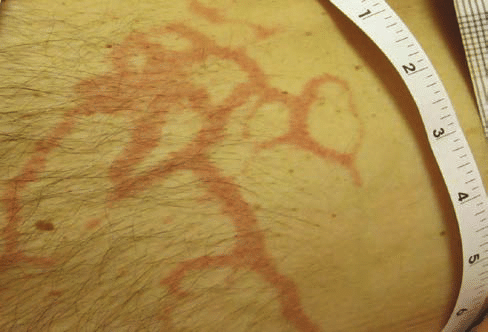
\includegraphics[width=\linewidth]{img/Atypical-reaction.png}
            \caption{Reazione atipica dopo la somministrazione di Bortezomib}
            
    \end{subfigure}
    \begin{subfigure}[b]{0.4\textwidth}
        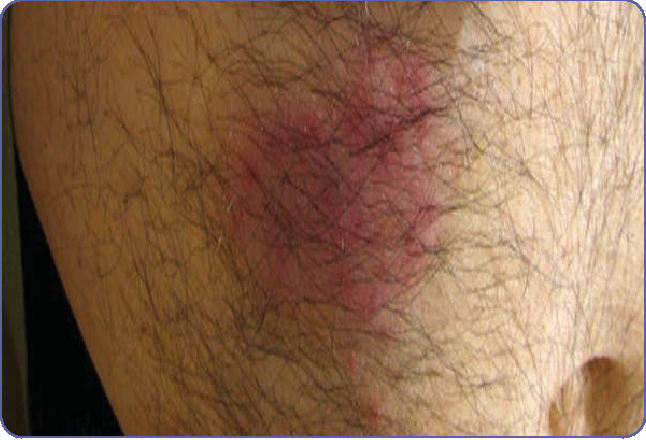
\includegraphics[width=\linewidth]{img/bortreaction.png}
        \caption{Reazione al Bortezomib dopo somministrazione per via sottocutanea}
      
\end{subfigure}
\end{center} 
    \caption{}
    \cite{{BORTEZOMIB}}
\end{figure}

\begin{figure}[H]
    \begin{center}
    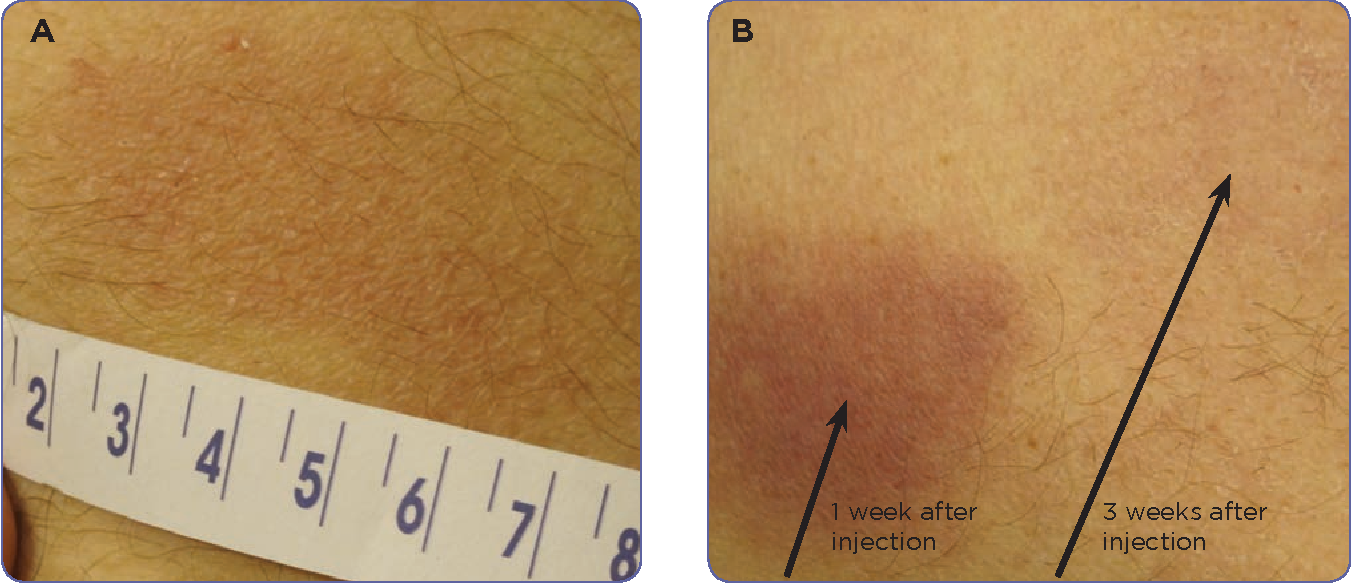
\includegraphics[width=0.7\columnwidth]{img/bortezomibreaction.png}
    \vspace{-3mm}
    \end{center}
    \caption{ Reazione al Bortezomib
    \cite{BORTEZOMIB}}
   
\end{figure}

L’infermiere è responsabile della somministrazione di Bortezomib per via sottocutanea e deve osservare,
attraverso una serie di step, tutti gli accorgimenti necessari per ridurre al minimo la probabilità di sviluppare 
reazioni avverse.\\ 
Nella scelta del sito di iniezione più adatto, bisogna ricordare che non ci sono evidenze che raccomandano l’iniezione 
nella regione deltoidea che, pertanto, non deve essere adoperata. Non deve essere altresì impiegata la zona periombelicale.
Evitare zone in cui si evidenziano rossore, calore, 
tumefazione, noduli, cute non integra, escoriazioni e segni di infiammazione. 
Ruotare le sedi di iniezione e documentare in cartella la sede utilizzata, in modo da usarne 
un’altra per la successiva somministrazione\cite{BORTNURSES}.

\begin{figure}[H]
    \begin{center}
    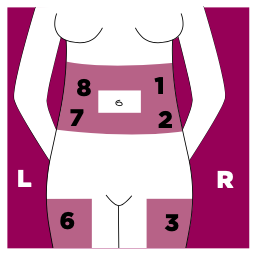
\includegraphics[width=0.3\columnwidth]{img/SEDI.png}
    \vspace{-3mm}
    \end{center}
    \caption{ Sedi di iniezione di Bortezomib per via sottocutanea
    \cite{BORTEZOMIB}}

\end{figure}

La tecnica di iniezione prevede di sollevare la plica cutanea prestando attenzione a sollevare il tessuto 
sottocutaneo, ma non quello muscolare (Figura \ref{fig:FIGURE_3.6}). 
Il volume massimo iniettabile mediante questa via è comunque di 2 mL.

\begin{figure}[H]
    \begin{center}
    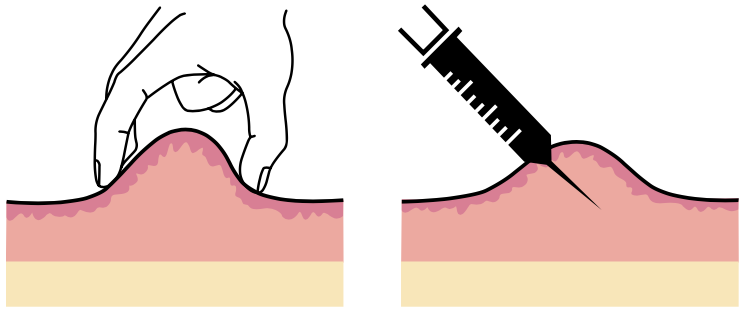
\includegraphics[width=0.5\columnwidth]{img/PLICA.png}
    \vspace{-3mm}
    \end{center}
    \caption{ Tecnica di iniezione con la plica cutanea
    \cite{BORTEZOMIB}}
    \label{fig:FIGURE_3.6}
\end{figure}

La scelta dell’ago appropriato è inoltre importante. Un ago da 26G è indicato per la somministrazione con un angolo di
90°, mentre se si opta per un angolo di 45° bisognerà usare un ago più piccolo per non incorrere nel rischio di 
penetrare nel tessuto muscolare\cite{BORTNURSES}.\\
Per la somministrazione di Bortezomib per via sottocutanea, risulta appropriata la tecnica "air sandwich" 
(Figura \ref{fig:FIGURE_3.7}),
da non usare invece per la via di somministrazione endovenosa. La tecnica prevede di aspirare 0.5-1 mL 
di aria nella siringa, che non deve essere rimossa, ma viene utilizzata per ridurre l'irritazione da parte del farmaco e 
per garantire la somministrazione dell'intera dose. L'iniezione deve essere lenta, con pause di circa 10 secondi. 
Al termine rimuovere l'ago e applicare una leggera pressione senza strofinare\cite{BORTNURSES}.

\begin{figure}[H]
    \begin{center}
    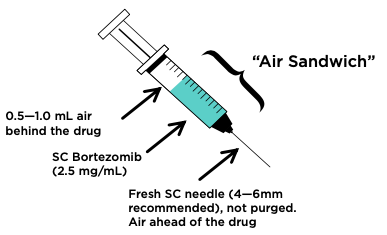
\includegraphics[width=0.5\columnwidth]{img/SIRINGA.png}
    \vspace{-3mm}
    \end{center}
    \caption{ Tecnica "air sandwich" per la somministrazione di Bortezomib per via sottocutanea
    \cite{BORTEZOMIB}}
    \label{fig:FIGURE_3.7}
\end{figure}

Bisogna educare il paziente riguardo il trattamento di possibili reazioni del sito di iniezione: 
possono essere assunti antistaminici per via orale, è raccomandata, dopo quattro ore dall’iniezione, 
l’applicazione per via topica di impacchi freddi, creme antistaminiche o cortisoniche;
applicarle prima potrebbe provocare dei cambiamenti nella farmacocinetica\cite{BORTEZOMIB}.\\
La neuropatia periferica è il principale effetto collaterale correlato alla somministrazione di Bortezomib, 
ma numerosi sono gli effetti collaterali che ne derivano: trombocitopenia, infezione, ipotensione, disturbi 
gastrointestinali, tumor lysis syndrome (TLS), problemi a livello cardiaco e polmonare, posterior reversible 
encephalopathy syndrome (PRES)\cite{BORTNURSES}.

\subsection{Inibitori del checkpoint immunitario o immune checkpoint inhibitors}

Il sistema immunitario possiede dei checkpoint, che hanno la funzione di impedire alle cellule immunitarie normali di 
attaccare le cellule sane dell’organismo. Le cellule cancerose spesso approfittano di questo meccanismo, per eludere il 
sistema immunitario e sfuggire al suo controllo.\\ 
Pembrolizumab è un farmaco che agisce andando a bloccare questi checkpoint, in modo che il sistema immunitario 
diventi responsivo verso le cellule cancerose. Tale farmaco viene usato per le forme recidive e refrattarie di linfoma 
primitivo a cellule B del mediastino\cite{IMMUNOTP}.

\subsection{Immunomodulatori o immunomodulating drugs}

Gli immunomodulatori sono farmaci come Talidomide e Lenalidomide, somministrati per via orale, per il trattamento di 
alcuni tipi di linfoma, dopo il tentativo fallito di altri approcci terapeutici\cite{MASSIVEBIO}.
Questi farmaci vanno a stimolare il sistema immunitario e possono contribuire al rallentamento della crescita di 
cellule cancerose.\\
Sono farmaci comunque non privi di effetti collaterali, come una bassa conta di globuli bianchi, che aumenta il 
rischio di sviluppare infezioni e neuropatia; Talidomide, inoltre, espone il paziente ad un maggior rischio di trombosi 
venosa profonda, fatigue e stipsi\cite{IMMUNOTP}.

\section{Trapianto di cellule staminali emopoietiche}

Le cellule staminali emopoietiche vengono prodotte nel midollo osseo, il quale si trova all’interno delle ossa; 
nel midollo osseo esse sono ancora cellule immature, è quando lo abbandonano e migrano nel sangue che si 
differenziano nei vari tipi cellulari: globuli rossi, globuli bianchi e piastrine. 
Questo processo è noto come ematopoiesi (Figura \ref{fig:FIGURE_3.14}) \cite{TRAPIANTO}.\\
Il trapianto di cellule staminali emopoietiche viene usato come approccio terapeutico nel linfoma non-Hodgkin, per 
poter somministrare alte dosi di chemioterapia con l'intento di distruggere le cellule cancerose, per poi introdurre 
nell’organismo, delle cellule staminali sane, che vadano a moltiplicarsi e a rigenerare il sistema immunitario.

\begin{figure}[H]
    \begin{center}
    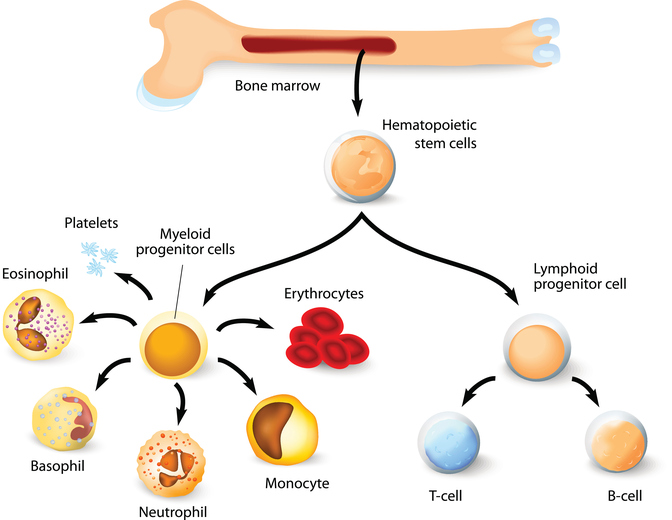
\includegraphics[width=0.5\columnwidth]{img/transplant.jpeg}
    \vspace{-3mm}
    \end{center}
    \caption{Il processo di ematopoiesi: come nascono e si differenziano i 
    vari tipi cellulari da una cellula staminale emopoietica
    \cite{img35}}
    \label{fig:FIGURE_3.14}
\end{figure}

Il trapianto di cellule staminali può essere autologo (il paziente è anche il donatore delle cellule staminali) 
o allogenico (il donatore può essere un familiare compatibile o un donatore volontario compatibile selezionato da una 
banca dati)\cite{LLS}.\\
Il trapianto autologo di cellule staminali emopoietiche, è il trattamento standard di elezione per le forme recidive e 
refrattarie di linfoma non-Hodgkin a cellule B\cite{TRANS} e per le recidive di forme indolenti.\\ 
Il trapianto allogenico, invece, è un’alternativa di trattamento, che può essere considerata per pazienti giovani con forme 
indolenti di LNH, che presentano caratteristiche di aggressività\cite{LLS}.\\
Il paziente, deve essere prima valutato, per verificare che sia candidabile al trapianto. 
Bisogna considerare il tipo di malattia e lo stadio, le condizioni generali del paziente, i trattamenti cui è stato 
sottoposto in precedenza, la probabilità di riuscita del trapianto, in termini di risposta da parte della malattia, 
oltre a una serie di esami: RX torace, ECG, ecocardiogramma, valutazione della funzionalità polmonare, TC o RMN, 
esami ematici per la valutazione dell’ematocrito, conta leucocitaria, screening per HIV, citomegalovirus (CMV), 
virus dell’epatite B (HBV); biopsia osteo-midollare (BOM), puntura lombare, esami delle urine ed ematici per la 
valutazione della funzionalità renale; valutazione con dentista e dietista; valutazione psicologica; 
coinvolgimento del caregiver a supporto del paziente durante tutto il processo, educazione dello stesso per il 
post-trapianto, ad esempio per il riconoscimento delle complicanze precoci, assunzione della terapia, preparazione 
dei pasti e gestione della casa, soprattutto per quanto riguarda la pulizia e la disinfezione\cite{LLS},\cite{STEMCELLS}.

\section{Fonti di cellule staminali emopoietiche}

Le cellule staminali emopoietiche possono essere raccolte dal midollo osseo, dal sangue periferico o dal sangue del 
cordone ombelicale.\\ 
Le cellule staminali vengono prelevate in genere dal midollo osseo delle creste iliache, in quanto ne contengono un 
numero elevato. La procedura si esegue in sala operatoria, ha la durata di circa 1-2 ore e il donatore è sottoposto 
ad anestesia generale. Dopo alcune ore di osservazione, il donatore viene dimesso nella stessa giornata
o il giorno seguente. L’organismo rigenera le nuove cellule in circa 4-6 settimane\cite{STEMCELLS}.\\ 
Non è una procedura che comporta dei rischi per il donatore e l’insorgenza di complicanze è rara; resta comunque 
un’operazione chirurgica e talvolta possono verificarsi reazioni all’anestesia, danni ai 
nervi o ai muscoli, infezione e dolore nel punto di inserzione dell’ago. 
Sintomi invece comuni dopo la procedura possono essere: dolore alla schiena, ematomi, iniziale difficoltà a camminare, 
stanchezza e debolezza, che si risolvono in qualche giorno\cite{STEMCELLS}.\\ 
Quando si è prelevato un quantitativo sufficiente di midollo, (generalmente il 10\% del midollo del donatore), 
questo viene filtrato e poi adeguatamente criopreservato, per poi essere scongelato quando deve essere somministrato 
al ricevente, per via endovenosa\cite{STEMCELLS}.
Per evitare l’anemia, conseguente al fatto che viene prelevato circa un litro di midollo osseo 
(700-1000 ml), al donatore, circa due settimane prima della donazione, viene prelevata una sacca di sangue, 
che gli sarà trasfusa durante la procedura\cite{TRAPIANTO}.\\

Nel sangue periferico, non è presente un numero elevato di cellule staminali; per questo motivo, qualche 
giorno prima del prelievo vengono somministrati farmaci che stimolano la produzione di cellule e la loro 
migrazione nel sangue periferico. Il sangue viene poi prelevato e filtrato tramite aferesi, per separare le cellule 
staminali dal resto delle cellule. Questo  processo dura circa 2-4 ore. Per ottenere un quantitativo adatto di cellule,
questo passaggio può essere ripetuto anche per alcuni giorni. 
Le cellule vengono poi congelate e sono pronte per la fase successiva: la somministrazione per via endovenosa\cite{STEMCELLS}.\\

Il sangue del cordone ombelicale è il sangue che resta nel cordone e nella placenta al momento del parto. 
Esso contiene numerose cellule staminali, che possono essere prelevate e conservate. 
È una procedura che non comporta alcun rischio per il neonato o la madre. 
Alcuni genitori decidono di donare le cellule staminali del cordone ombelicale ad una banca pubblica, altri invece 
possono decidere di conservarlo in una banca privata così da averlo se in futuro un membro della famiglia o un figlio 
dovesse averne bisogno. Nel fare ciò bisogna considerare però, che un solo cordone non ha cellule a sufficienza per un 
adulto, non è detto che la malattia che si potrebbe sviluppare, possa essere trattata con un trapianto autologo o 
comunque usando quel cordone ombelicale, che dopo tanti anni potrebbe non risultare una terapia efficace, oltre 
all’elevato costo per la conservazione di un cordone\cite{STEMCELLS}.

\section{Trapianto autologo di cellule staminali emopoietiche}

Nel trapianto autologo, sono le stesse cellule staminali del paziente ad essere utilizzate per l’infusione. 
Questo processo, segue una serie di fasi (Figura \ref{fig:FIGURE_3.15}).\\
Inizialmente si favorisce la mobilizzazione, cioè la produzione, di cellule staminali emopoietiche e la 
loro migrazione dal midollo osseo al sangue. Vengono somministrati farmaci detti fattori di crescita granulocitari, 
per via sottocutanea, per circa 4-6 giorni\cite{TRAPIANTO}. Un esempio è Filgrastim, che non è privo di effetti 
collaterali, ma che comunque passano dopo la fine delle somministrazioni; si possono manifestare mal di testa, 
dolore alle ossa, nausea, disturbi del sonno, febbricola e stanchezza\cite{STEMCELLS}.\\
La seconda fase è di prelievo delle cellule staminali, tramite vena periferica, oppure dalle creste iliache delle 
ossa del bacino, in caso di prelievo dal midollo.\\ 
Abbiamo successivamente la fase di aferesi, in cui le cellule staminali vengono isolate dal resto delle cellule, 
le quali invece vengono restituite al donatore.\\ 
La fase di aferesi, è seguita dalla fase di condizionamento (della durata di 3-9 giorni), che prevede la 
somministrazione di chemioterapia e/o radioterapia a dosi elevate, con lo scopo di eliminare, 
per quanto possibile, le rimanenti cellule tumorali. In questo modo anche 
le cellule staminali presenti nel midollo vengono meno. Trascorse 48-72 ore dalla fine del condizionamento, 
al paziente vengono somministrate le cellule staminali, previo scongelamento, alla temperatura di 37°C, 
in vena centrale\cite{TRAPIANTO}.\\
L’organismo, a questo punto, attraversa una fase di aplasia, ovvero che il numero di globuli rossi, globuli bianchi e 
piastrine, diminuisce notevolmente per via della terapia di condizionamento. La durata di questa fase dipende 
dalla malattia, dai farmaci impiegati e generalmente si può protrarre per circa 2-3 settimane\cite{TRAPIANTO}, 
periodo in cui il paziente è maggiormente suscettibile ad infezioni, per via della bassa conta di globuli bianchi, 
anemia, causata dal deficit di globuli rossi e maggior rischio di sanguinamento per via della trombocitopenia\cite{LLSBLOOD}.\\
La fase di ricostituzione ematologica che segue l’aplasia, prevede che il midollo osseo, grazie alle cellule infuse, 
inizi a produrre nuove cellule staminali\cite{TRAPIANTO}.
È una fase dalla durata variabile, può impiegare circa 3-4 settimane o anche di più, periodo in cui il paziente 
è sottoposto a frequenti controlli ematici, per verificare che il midollo abbia iniziato a produrre nuove cellule\cite{LLSBLOOD}.\\

Il trapianto autologo di cellule staminali emopoietiche ha come aspetto positivo che il paziente riceve le sue 
stesse cellule, quindi non c’è rischio di rigetto delle cellule trasfuse.\\ 
Uno dei rischi di questo tipo di trapianto è però che le cellule trasfuse non vadano nel midollo osseo e non 
sviluppino un numero sufficiente di nuove cellule. Un altro svantaggio è che nella fase di prelievo delle cellule, 
potrebbero venir prelevate anche cellule cancerose, che verranno reinfuse nuovamente al paziente; inoltre può 
verificarsi che, nonostante il trapianto, le cellule cancerose riescano comunque ad evadere dall’attacco 
del sistema immunitario\cite{STEMCELLS}.

\begin{figure}[H]
    \begin{center}
    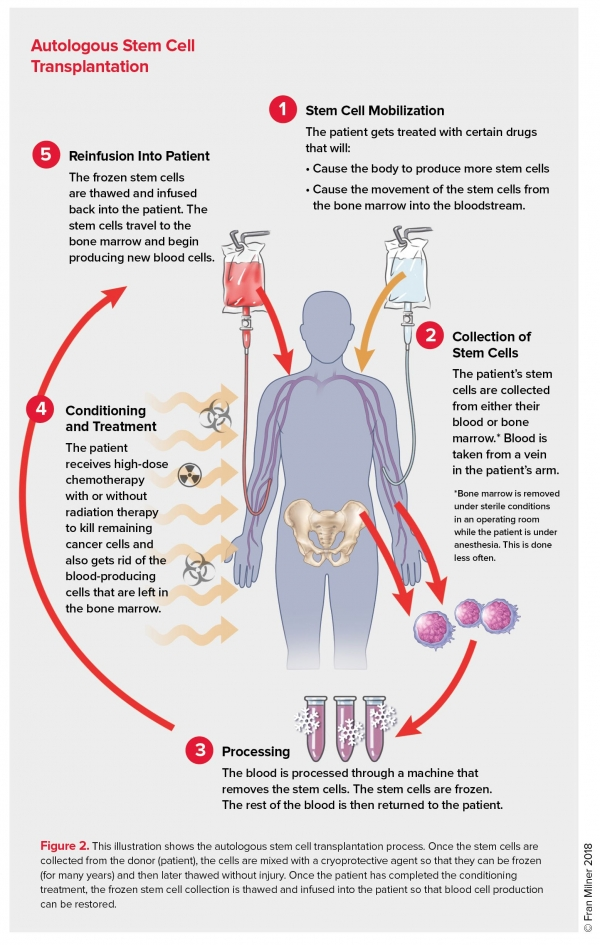
\includegraphics[width=0.7\columnwidth]{img/AUTOLOGO.jpeg}
    \vspace{-3mm}
    \end{center}
    \caption{Fasi del processo di prelievo e somministrazione di cellule staminali emopoietiche nel trapianto autologo
    \cite{LLSBLOOD}}
    \label{fig:FIGURE_3.15}
\end{figure}

\section{Trapianto allogenico di cellule staminali emopoietiche}

Il trapianto allogenico, segue lo stesso principio del trapianto autologo; in questo caso, le cellule staminali emopoietiche, 
vengono prelevate da un donatore, che può essere un parente, oppure un donatore volontario.\\ 
Prima del trapianto, il paziente è sottoposto al processo di condizionamento (somministrazione di elevate dosi di 
chemioterapia e/o radioterapia), con lo scopo di distruggere le cellule cancerose presenti nell’organismo, 
indebolire il sistema immunitario, per cercare di ridurre il rischio di rigetto del trapianto e permettere alle 
cellule staminali, di raggiungere, tramite il circolo sanguigno, il midollo osseo, da cui inizierà la produzione 
di nuove cellule.\\
Un aspetto positivo del trapianto allogenico, che non si verifica nel trapianto autologo, è il graft-versus-tumor 
effect (GVT), ovvero che i globuli bianchi del donatore, riconoscono come estranee le restanti cellule tumorali 
del ricevente e le attaccano selettivamente\cite{LLSBLOOD}.\\ Nella figura \ref{fig:FIGURE_3.10}, 
sono riportate le fasi che caratterizzano il trapianto allogenico.

\subsection{Trapianto non-mieloablativo o reduced-intensity}

Un altro tipo di trapianto allogenico, è quello definito non-mieloablativo o mini allotrapianto o ancora trapianto a 
ridotta intensità (reduced-intensity). Questo tipo di trapianto, rappresenta un’alternativa per pazienti non 
candidabili al trapianto allogenico, a causa della loro età e delle condizioni di salute. In questo tipo di trapianto, 
il condizionamento prevede la somministrazione di chemioterapia e/o radioterapia a dosi più basse\cite{LLSBLOOD}.\\
L’obiettivo di questo trapianto, è quello di sfruttare il graft-versus-tumor effect, in cui le cellule del donatore, 
nel midollo osseo, stimolano la produzione di globuli bianchi, che vadano ad attaccare le cellule tumorali, con il 
vantaggio di avere un condizionamento più lieve e di conseguenza, la conta delle cellule ematiche 
non scende come nel trapianto standard\cite{STEMCELLS}.\\
Nonostante gli aspetti positivi, gli aspetti negativi accomunano sia il trapianto allogenico che il mini allotrapianto.\\
Quando si decide per un allotrapianto, trovare un donatore con un’elevata compatibilità è molto importante, 
per cercare di prevenire complicanze di rigetto nel post-trapianto. In genere si inizia a cercare tra i parenti, 
altrimenti si opta per un donatore scelto da banche di midollo osseo\cite{TRAPIANTO}.

\begin{figure}[H]
    \begin{center}
    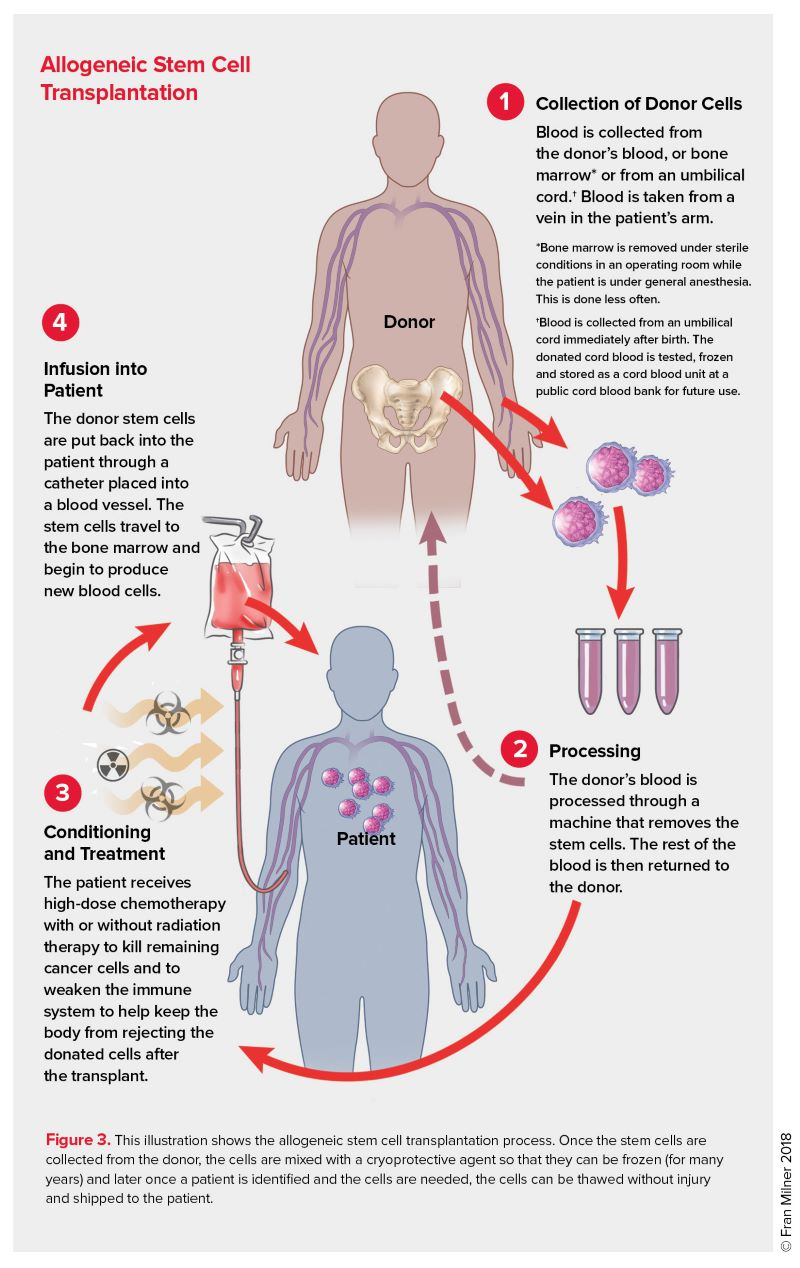
\includegraphics[width=0.7\columnwidth]{img/ALLOGENICO.jpg}
    \vspace{-3mm}
    \end{center}
    \caption{Fasi del trapianto allogenico di cellule staminali emopoietiche
    \cite{LLSBLOOD}}
    \label{fig:FIGURE_3.10}
\end{figure}

\section{Complicanze correlate al trapianto di cellule staminali emopoietiche}

La complicanza più comune e più temuta, al trapianto allogenico di cellule staminali emopoietiche e anche al mini 
allotrapianto è la reazione da trapianto contro l’ospite (graft-versus-host disease, GVHD). Questa complicanza, 
che può essere lieve, moderata, severa e in alcuni casi anche potenzialmente mortale, si verifica quando le cellule 
del donatore, riconoscono come estranee le cellule del ricevente e iniziano ad attaccarle. Un’elevata compatibilità 
tra donatore e ricevente, nonché l’utilizzo di terapie per prevenire la GVHD possono aiutare, ma in alcuni casi non 
impediscono ugualmente lo sviluppo di questa complicanza.\\ 
La GVHD può essere acuta o cronica, i sintomi possono coinvolgere diversi organi e apparati (Figura \ref*{fig:FIGURE_3.17})
e i pazienti possono sviluppare una delle due, entrambe o nessuna\cite{LLSBLOOD}.

\begin{figure}[H]
    \begin{center}
    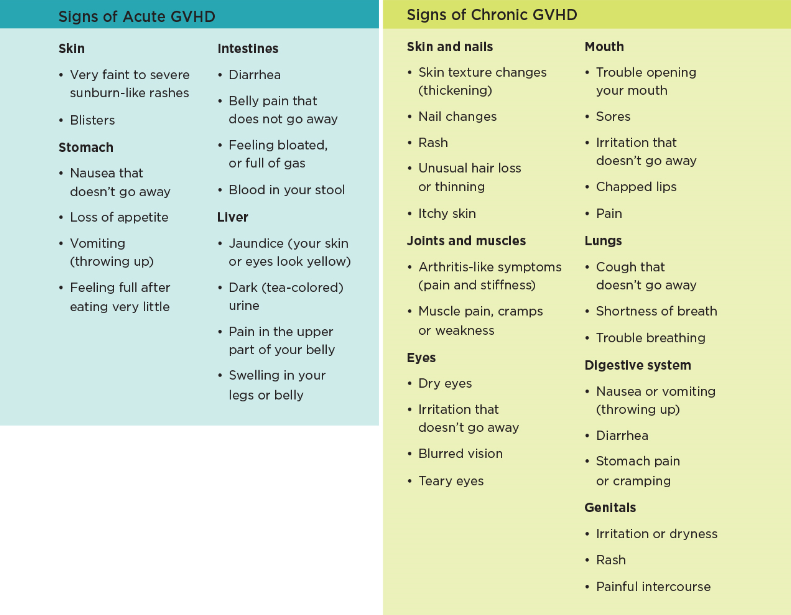
\includegraphics[width=0.9\columnwidth]{img/SignsGVHD.png}
    \vspace{-3mm}
    \end{center}
    \caption{Sintomi di GVHD acuta e cronica
    \cite{img38}}
    \label{fig:FIGURE_3.17}
\end{figure}

La GVHD acuta, generalmente, insorge nei primi 100 giorni post-trapianto, con sintomi che possono interessare pelle, 
tratto gastrointestinale e fegato. Per prevenire la GVHD vengono somministrati degli immunosoppressori, come 
metotrexato, ciclosporina, tacrolimus e alcuni anticorpi monoclonali. 
Nonostante ciò una GVHD in forma lieve può comunque svilupparsi\cite{STEMCELLS}.\\
La terapia sistemica di prima linea per una GVHD acuta prevede la somministrazione di metilprednisolone o prednisone\cite{GVHD}.\\
La GVHD cronica, solitamente, si sviluppa tra 3 e 6 mesi dopo il trapianto, può coinvolgere uno o più organi. 
Se i sintomi sono lievi, possono essere trattati con osservazione e terapia topica, in caso di sintomi gravi, si rende 
necessaria una terapia endovenosa sistemica con farmaci immunosoppressori, che però aumentano il rischio 
di contrarre infezioni\cite{STEMCELLS}.\\

Nel post-trapianto aumenta per il paziente il rischio di contrarre infezioni, per la presenza del basso numero 
di globuli bianchi nel sangue. Per prevenire il rischio di infezioni, verranno somministrati farmaci antibiotici, 
antivirali ed antifungini.\\ Se il paziente riceve delle visite, i visitatori devono eseguire il lavaggio delle mani, 
non sono ammessi ad entrare se presentano sintomi influenzali e non possono portare fiori o piante in quanto 
fonte di microrganismi. È importante prestare attenzione anche ai cibi: frutta e verdura devono essere 
lavate accuratamente; cibi come carne, pesce e uova devono essere consumati ben cotti e questi accorgimenti 
sono da mantenere anche dopo la dimissione, fino a quando il sistema immunitario non sarà più indebolito\cite{LLSBLOOD}.\\
In questa fase, infezioni generalmente innocue, possono risultare pericolose per i pazienti trapiantati. 
La polmonite Pneumocystis carinii (PCP), causata dalla \emph{pneumocystis pneumonia} o \emph{pneumocystis jirovecii} (PJP), 
è comune nei pazienti immunodepressi.\\
Prima del trapianto, il medico esegue dei controlli, per il ricevente e per il donatore, in quanto alcune 
infezioni, potrebbero riattivarsi: è il caso del citomegalovirus (CMV), asintomatico in soggetti sani, 
può essere causa di polmonite severa in pazienti immunodepressi\cite{STEMCELLS}.\\
A causa dell’elevato rischio di sviluppare infezioni, il paziente viene monitorato nel caso manifesti sintomi come 
febbre, tosse, dispnea e diarrea; vengono eseguiti esami ematici e si predispone un regime di isolamento, con 
ingressi nella stanza controllati e mirati, che prevedono di indossare il camice monouso, le sovrascarpe, 
la mascherina e gli occhiali protettivi.
Anche dopo la fase di ricostituzione ematologica, è un rischio presente fino a 6-12 mesi dopo il trapianto, e questo 
tempo si allunga se il paziente sviluppa una GVHD\cite{STEMCELLS}.\\

Il basso numero di globuli rossi aumenta il rischio di anemia, che si presenta con fatigue, debolezza e dispnea; 
il paziente potrebbe necessitare di trasfusioni di unità di globuli rossi concentrati\cite{LLSBLOOD}.\\
A causa della trombocitopenia, è esposto ad un maggior rischio di sanguinamento e potrebbe 
rendersi necessaria una trasfusione di piastrine\cite{LLSBLOOD}.\\

Effetti collaterali che insorgono nel post-trapianto, causati dal condizionamento con chemioterapia e/o radioterapia 
possono essere: nausea e vomito, diarrea, stipsi, stanchezza, febbre, dolore, presenza di sangue nelle urine, 
perdita di capelli, mucositi, eruzioni cutanee, problematiche a carico di cuore, polmoni e nervi\cite{LLSBLOOD}.\\
Si possono verificare anche una ridotta funzionalità tiroidea, cataratta, problemi di infertilità sia nell’uomo 
che nella donna, menopausa precoce nella donna.\\
Si cerca di prevenire l’insorgenza di nausea e vomito mediante la somministrazione di antiemetici, talvolta 
può essere necessario combinare più antiemetici o sostituirli se non efficaci. 
Nonostante ciò è un rischio che non si può completamente prevenire, ma sicuramente è da prevenire prima che insorga\cite{STEMCELLS}.\\

Un’altra complicanza al trapianto, è il fallimento di innesto o graft failure, che può verificarsi quando le cellule 
trapiantate del donatore, non raggiungono il midollo osseo per produrre nuove cellule. È una complicanza molto rara 
nel trapianto autologo, invece è più frequente nel trapianto allogenico, soprattutto se non c’è una buona 
compatibilità tra donatore e ricevente. In tal caso si può pensare di procedere con un secondo trapianto allogenico, 
dallo stesso donatore o da un donatore differente\cite{LLSBLOOD}.\\

La malattia linfoproliferativa post-trapianto (Post-Transplant Lymphoproliferative Disorders, PTLD) è una forma di 
linfoma, caratterizzata da una crescita incontrollata dei linfociti dopo il trapianto allogenico di cellule staminali 
emopoietiche. In genere insorge dopo un anno dal trapianto, e rappresenta un rischio maggiore, in caso di incompatibilità 
tra donatore e ricevente e immunosoppressione.\\
L’insorgenza di PTLD è legata al fatto che i linfociti T non riescono ad eliminare le cellule contenenti 
virus e quindi nel caso in cui sia presente il virus di Epstein-Barr (EBV) esso causa un’infezione fuori controllo 
a causa della debolezza del sistema immunitario. Il trattamento non è standard, in genere si cessa il trattamento 
con gli immunosoppressori, si può ricorrere ad una trasfusione di globuli bianchi per potenziare il sistema 
immunitario, somministrare farmaci anti-virali e anticorpi come Rituximab, che va ad uccidere le cellule B infettate 
dal virus EBV\cite{STEMCELLS}.

\subsection{Criteri per la dimissione del paziente trapiantato}

Affinché il paziente possa essere dimesso dopo il trapianto, devono verificarsi le seguenti condizioni: 
non deve aver presentato febbre nelle ultime 48 ore; 
nausea, vomito e diarrea sono controllati; il paziente nelle ultime 48 ore è riuscito ad assumere 
farmaci; sono assenti segni di infezione; la conta dei neutrofili è almeno 500-1000 mm/3 di sangue; l’ematocrito è 
almeno 25-30\%; la conta delle piastrine è almeno 15.000-20.000 mm/3 di sangue; è assicurata la presenza del 
caregiver che supporti il paziente nei suoi bisogni, che sia adeguatamente educato nel riconoscimento precoce di 
eventuali complicanze e che si occupi di accompagnare il paziente ai vari controlli, piuttosto 
frequenti nel primo periodo post-operatorio\cite{STEMCELLS}.





















